\hypertarget{_s_c_p_i__parser_8h}{\section{scpi/\-S\-C\-P\-I\-\_\-parser.h File Reference}
\label{_s_c_p_i__parser_8h}\index{scpi/\-S\-C\-P\-I\-\_\-parser.\-h@{scpi/\-S\-C\-P\-I\-\_\-parser.\-h}}
}
This graph shows which files directly or indirectly include this file\-:\nopagebreak
\begin{figure}[H]
\begin{center}
\leavevmode
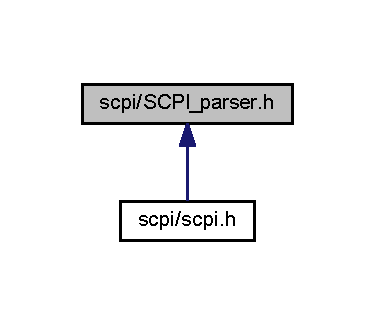
\includegraphics[width=180pt]{_s_c_p_i__parser_8h__dep__incl}
\end{center}
\end{figure}


\subsection{Detailed Description}
The parser is the logical portion of a device that takes D\-A\-Bs, E\-N\-D messages and G\-E\-T messages from the input buffer and analyses them by separating out the various I\-E\-E\-E488.\-2 syntactic elements into an internal representation which is sent to the execution control. The parser also generates the eom and query messages when it recognises these syntactic element.

A $ \langle$ P\-R\-O\-G\-R\-A\-M M\-E\-S\-S\-A\-G\-E $ \rangle$ or $ \langle$ P\-R\-O\-G\-R\-A\-M M\-E\-S\-S\-A\-G\-E U\-N\-I\-T $ \rangle$ is considered \char`\"{}parsed\char`\"{} when it has been analysed by the parser and the parser is ready to continue analysing other $ \langle$ P\-R\-O\-G\-R\-A\-M M\-E\-S\-S\-A\-G\-E U\-N\-I\-T $ \rangle$ elements.

This file should not need to be edited by the user 